        %%******************************************%%
        %%                                          %%
        %%        Modello di tesi di laurea         %%
        %%            di Andrea Giraldin            %%
        %%                                          %%
        %%             2 novembre 2012              %%
        %%                                          %%
        %%******************************************%%

\begin{document}
    \frontmatter
    \begin{titlepage}
    \begin{center}
        \begin{LARGE}
            \textbf{\myUni}\\
        \end{LARGE}

        \vspace{10pt}

        \begin{Large}
            \textsc{\myDepartment}\\
        \end{Large}

        \vspace{10pt}

        \begin{large}
            \textsc{\myFaculty}\\
        \end{large}

        \vspace{30pt}
        \begin{figure}[htbp]
            \centering
            
\includegraphics[height=6cm]{unipd-logo}
        \end{figure}
        \vspace{30pt}

        \begin{LARGE}
            \textbf{\myTitle}\\
        \end{LARGE}

        \vspace{10pt}

        \begin{large}
            \textsl{\myDegree}\\
        \end{large}

        \vspace{40pt}

        \begin{large}
            \begin{flushleft}
                \textit{Relatrice}\\
                \vspace{5pt}
                \profTitle\ \myProf
            \end{flushleft}

            % You can tweak the spacing to have professor and student names on the same line
            % useful if the page is broken by a long thesis title and you need more space
            % \vspace{-52pt}

            \begin{flushright}
                \textit{Laureando}\\
                \vspace{5pt}
                \myName \\
                \vspace{5pt}
                Matricola: \myMatricola
            \end{flushright}
        \end{large}

        \vspace{28pt}

        \line(1, 0){338} \\
        \begin{normalsize}
            \textsc{Anno Accademico \myAA}
        \end{normalsize}
    \end{center}
\end{titlepage}

    \clearpage
\phantomsection
\thispagestyle{empty}

\hfill
\vfill

\noindent\myName: \textit{\myTitle,}
\myDegree,
\textcopyright\ \myTime.

    \cleardoublepage
\phantomsection
\thispagestyle{empty}
\pdfbookmark{Dedica}{Dedica}

\vspace*{3cm}

\begin{center}
    Leave a Little Sparkle wherever you go. \\ \medskip
\end{center}

\medskip

\begin{center}
    Dedicato a tutti coloro che ci sono stati vicini nei momenti più difficili.
\end{center}

    \cleardoublepage
\phantomsection
\pdfbookmark{Sommario}{Sommario}
\begingroup
\let\clearpage\relax
\let\cleardoublepage\relax
\let\cleardoublepage\relax

\chapter*{Sommario}

Il presente documento descrive il lavoro svolto durante il periodo di stage, della durata di circa trecento ore, dal laureando Marco Brugin presso l'azienda Sybclab S.r.L.
Gli obbiettivi da raggiungere sono stati:
in primo luogo è stata richiesta la comprensione dei vantaggi e degli overhead portati da una architettura Event Driven,
in secondo luogo è stata richiesta la comprensione e implementazione di una data pipeline con il trattamento dei dati tramite Apache Kafka e Apache Druid ed infine la comprensione e la gestione gestione delle Time Series e dei Column-based Databases.
Il prototipo sviluppato presenterà una architettura distribuita, ad alta affidabilità, scalabile e resiliente, eseguibile tramite Docker Compose.
%\vfill

%\selectlanguage{english}
%\pdfbookmark{Abstract}{Abstract}
%\chapter*{Abstract}

%\selectlanguage{italian}

\endgroup

\vfill

    \cleardoublepage
\phantomsection
\pdfbookmark{Ringraziamenti}{ringraziamenti}

\begin{flushright}{
    \slshape
    ``Life is really simple, but we insist on making it complicated''} \\
    \medskip
    --- Confucius
\end{flushright}


\bigskip

\begingroup
\let\clearpage\relax
\let\cleardoublepage\relax
\let\cleardoublepage\relax

\chapter*{Ringraziamenti}

\noindent \textit{Innanzitutto, vorrei esprimere la mia gratitudine al Prof. \myProf, relatore della mia tesi, per l'aiuto e il sostegno fornitomi durante la stesura del lavoro.}\\

\noindent \textit{Desidero ringraziare con affetto i miei genitori per il sostegno, il grande aiuto e per essermi stati vicini in ogni momento durante gli anni di studio.}\\

\noindent \textit{Ho desiderio di ringraziare poi i miei amici per tutti i bellissimi anni passati insieme e le mille avventure vissute.}\\
\bigskip

\noindent\textit{\myLocation, \myTime}
\hfill \myName

\endgroup

    \cleardoublepage
\pdfbookmark{\contentsname}{tableofcontents}
\setcounter{tocdepth}{2}
\tableofcontents
%\markboth{\contentsname}{\contentsname}
\clearpage

\begingroup
    \let\clearpage\relax
    \let\cleardoublepage\relax
    \let\cleardoublepage\relax

    % Figures list
    \phantomsection
    \pdfbookmark{\listfigurename}{lof}
    \listoffigures

    \vspace*{8ex}

    % Tables list
    \phantomsection
    \pdfbookmark{\listtablename}{lot}
    \listoftables

    \vspace*{8ex}
\endgroup

\cleardoublepage

    \cleardoublepage

    \mainmatter
    \chapter{Introduzione}
\label{cap:introduzione}
\section{Descrizione dell'azienda}
Sync Lab s.r.L. è una azienda italiana attiva nell'abito \gls{ict}{}, specializzata nello sviluppo e consulenza IT dal 2002 con sedi a 
Milano, Roma, Napoli, Verona e Como. È una azienda orientata verso la Business Innovation, finalizzata alla 
creazione di soluzioni innovative che abbracciano i nuovi paradigmi della trasformazione digitale.
Sync Lab possiede numerose certificazioni ISO LL-C per l'attestazione della 
qualità dei prodotti e servizi offerti. In particolare possiede le certificazioni 
ISO-9001 per la qualità dell'azienda, ISO-14001 per l'adozione quadro sistematico per l'integrazione delle pratiche a protezione dell'ambiente, ISO-27001 per la definizione di un \gls{sgsi}{}, ISO-45001 per l'adozione di un \gls{ohs}{}.
\\
Attualmente Sync Lab dal punto di vista dell'organico è composta da più 300 dipendenti e lavora per più di 150 clienti diretti e finali, tra i più rilevanti ci sono nomi come: TIM, Trenitalia, PosteItaliane, UniCredit, ENI, ENEL, Vodafone, Fastweb.
\\
Sync Lab è un'azienda che si pone come obiettivo quello di essere un punto di riferimento per i propri clienti nella realizzazione di prodotti e soluzioni innovative per diversi settori di mercato, come mostrato  tra i quali: Sanità, Industria, Energia, Telco, Finanza e Trasporti \& Logistica.\\
Lo spirito di Sync Lab è ampiamente rappresentato dal logo aziendale Figura \ref{figure:logo_azienda}, che rappresenta un'onda che si propaga in modo circolare, che simboleggia la capacità di adattarsi e di evolversi in modo continuo.\\


\begin{figure}[htbp]  
\centering
    
\includegraphics[width=0.5\textwidth]{images/introduzione/logo_azienda.png}
    \caption{Logo dell'aziedan Sync Lab s.r.L.}
    \label{figure:logo_azienda}
\end{figure}
\pagebreak
\section{Idea di fondo del progetto}
Oggigiorno la gestione e l'analisi di grandi moli di dati in tempo reale sta diventando fondamentale 
per le aziende che vogliono rimanere competitive sul mercato. \\ 
Per questo motivo è necessario utilizzare tecnologie e software che permettano di analizzare e archiviare 
i dati in modo efficiente e veloce. \\
D'altro canto, però, è necessario anche che queste tecnologie siano in grado di scalare in modo verticale e orizzontale in base al carico 
di lavoro da sostenere. Inoltre è necessario che queste tecnologie siano in grado di garantire un elevato livello affidabilità. \\
Per questo motivo Sync Lab ha deciso d' investire in un progetto di ricerca e sviluppo che ha come obiettivo quello di creare 
una \gls{Data Pipeline}{} in grado di garantire le caratteristiche sopra descritte. \\
L'azienda ha già a disposizione un sistema di raccolta dati in  real time, basato su Apache Kafka, che permette di ricevere dati da
diversi sistemi e applicazioni, ma vuole andarlo a integrare con un sistema di analisi in real time permetta di eseguire operazioni 
sui dati ricevuti prima di archiviarli. \\
Particolarmente importante dovrà essere la fase di analisi dei dati, in quanto dovrà essere possibile eseguire operazioni di aggregazione
per aumentare la successiva estrazione dei dati. 
\subsection{Il ruolo dello stagista}
Lo stagista ha un ruolo fondamentale in tale tipologia di progetto, infatti è colui che porta uno spirito d'innovazione e consolida il valore aggiunto 
aziendale. \\
Le attività che costituiscono il percorso che lo stagista ha intrapreso sono state elencate all'interno di un \textit{Piano di lavoro}, che ha aiutato il tutor 
aziendale designato da Sync Lab a guidare e valutare il lavoro svolto dallo stagista. \\
Inoltre al termine del periodo di stage, sotto la supervisione del tutor aziendale è stata pianificata una presentazione rivolta a tutti \textit{stakeholder} aziendali, mirata a 
mostrare i risultati ottenuti con le tecnologie utilizzate e mettere in risalto le potenzialità del prototipo sviluppato. D'altra parte tale presentazione è stata anche l'occasione 
per un confronto per far emergere eventuali criticità o difetti,  e miglioramenti da apportare al prototipo sviluppato.
\pagebreak
\section{Il progetto di stage}
\subsection{Descrizione del progetto}
Le attività descritte in questa tesi si basano sulla progettazione e realizzazione di un prototipo di \gls{Data Pipeline}{} in grado di ricevere dati in real time da un sistema di raccolta dati basato su Apache Kafka, eseguire operazioni di aggregazione con Apache Druid in modo efficiente per facilitarne la successiva estrazione, fornendo così in output dati pronti per l'analisi.\\
In generale una \gls{Data Pipeline}{} è costituita da tre elementi sostanziali: una origine, una o più fasi di trasformazione e una o più destinazioni.
Inoltre per facilitare le operazioni di deploy è richiesto che il prototipo sia eseguibile con Docker Compose. \\
Il progetto in sè fa parte di una rivoluzione tecnologica che Sync Lab sta portando avanti nel campo \gls{Data Processing}{} e \gls{Data Analytics}{}. \\
In particolare il progetto di stage si pone come obiettivo quello di andare ad analizzare le prestazioni di Apache Druid rispetto ad un classico database relazionale, come PostgreSQL, in termini di velocità di esecuzione delle query e di scalabilità in relazione alle funzionalità di aggregazione fornite da tale strumento. 
\subsection{Obiettivi formativi}
In generale lo stage ha come obiettivo quello di far acquisire allo stagista concetti fondamentali riguardanti: 
\begin{itemize}
    \item Container technology;
    \item Apache Kafka e le Event Driven Architecture, design publish/subscribe;
    \item Column Based Database e la relazione/confronto tra questi e i classici DB relazionali SQL e quelli
    Documentali;
    \item Middleware, \gls{Data Pipeline}{}, le architetture distribuite, scalabili e resilienti.
\end{itemize}
\subsection{Risultati attesi e Obiettivi fissati}
Sono riportati nella Tabella \ref{tab:Tabella1} i risultati attesi e gli obiettivi fissati per lo stage con rispettivo identificativo, importanza e breve descrizione.
L'identificativo (riportato in breve con “ID”) è la sigla che identifica ogni requisito e rispetta la seguente notazione [Importanza][Identificativo]. \\
L’importanza è indicata dalla sigla O oppure F ad indicare rispettivamente un obiettivo
obbligatorio oppure facoltativo; mentre l’identificativo è un numero incrementale che
segnala in modo univoco l’obiettivo o il risultato in esame.\\
\\
Ogni obiettivo è identificato, o risultato viene classificato secondo l'importanza in: 
\begin{list}{*}{}
    \item \textbf{Obbligatorio (O)}: obiettivo irrinunciabile, vincolante in quanto necessario per l'avanzamento del progetto;
    \item \textbf{Facoltativo (F)}: obiettivo utile ma non essenziale, che può essere soddisfatto solo se tutti gli obiettivi obbligatori sono stati raggiunti e il cui soddisfatto rende il progetto più completo.     
\end{list} 

 \begin{table}[htbp]
    \centering
    \caption{Tabella degli obiettivi}    
    \label{tab:Tabella1}
    \begin{tabularx}{\textwidth}{|c|c|X|}
        \hline
        \textbf{ID} & \textbf{Importanza} & \textbf{Descrizione} \\\hline
        O1 & Obbligatorio & comprensione e definizione di una piccola \gls{Data Pipeline}{}  che  preveda il trattamento dei dati
        tramite Apache Kafka e Apache Druid \\\hline
        O2 & Obbligatorio & comprensione dei vantaggi e degli overhead  che le Event Driven Architecture portano con
        sé\\\hline
        O3 & Obbligatorio & comprensione del pattern publisher/subscriber \\\hline
        O4 & Obbligatorio & set-up di un cluster Apache Kafka in ambiente  containerizzato \\\hline
        O5 & Obbligatorio & gestione delle Time Series e dei Column-based Databases \\\hline
        O6 & Obbligatorio & comprensione delle differenze tra i database relazionali  classici e i Column-based Databases\\\hline
        O7 & Obbligatorio &comprensione dell’impiego e utilità dei middleware \\\hline
        F1 & Facoltativo & produzione di documentazione e un pacchetto di configurazione  dell’ambiente di sviluppo e
        esecuzione  della \gls{Data Pipeline}{}\\\hline
        F2 & Facoltativo & produzione di documentazione che riporti  le differenze  di performance  tra Apache Druid e altri
         database relazionali classici per alcune  operazioni \gls{olap}{} \\\hline
        F3 & Facoltativo & realizzazione di una presentazione che illustri l’architettura  sviluppata  a personale di settore o
        Stakeholder \\\hline
    \end{tabularx} 

\end{table}

\pagebreak

\pagebreak
\subsection{Analisi preventiva dei rischi}
Durante la fase di analisi iniziale del progetto di stage, sono stati individuati i seguenti rischi, cui si è cercato di porre rimedio con le azioni di mitigazione indicate. \\
\begin{enumerate}
    \item \textbf{Inesperienza tecnologica}: il progetto prevede l'utilizzo di tecnologie con cui lo stagista non ha mai avuto a che fare. \\
    \textbf{Rischio}: Medio.\\
    \textbf{Soluzione}: Per mitigare tale rischio, è stato previsto un periodo di ambientamento e delle tecnologie coinvolte, in modo da poter affrontare il progetto con maggiore consapevolezza.
    \item \textbf{Scelte errate nella progettazione dell'architettura}: il progetto prevede la progettazione di un'architettura complessa, con molte componenti interagenti tra loro. \\
    \textbf{Rischio}: Alto.\\
    \textbf{Soluzione}: Per mitigare tale rischio, è stato previsto un periodo di analisi e progettazione dell'architettura, con il supporto del tutor aziendale, in modo da poter ovviare tale rischio.
    \item \textbf{Prestazioni insufficienti delle macchine a disposizione}: il progetto prevede l'impiego di tecnologie che richiedono un elevato dispendio di risorse. Tale fattore se non tenuto in considerazione potrebbe portare a risultati penalizzanti. \\
    \textbf{Rischio}: Alto.\\
    \textbf{Soluzione}: Per mitigare tale rischio, è stato prevista la configurazione degli strumenti utilizzati in modo tale da utilizzare al meglio le risorse a disposizione.
\end{enumerate}    
\subsection{Obiettivi personali}
Nonostante la realizzazione del progetto sia l'obiettivo principale, gli obbiettivi da perseguire riguardano essenzialmente l'acquisizione di competenze e conoscenze, dall'ambiente ospitante, piuttosto che la realizzazione del prodotto in sè. \\

\noindent In particolare, gli obiettivi personali sono:
\begin{list}{*}{}
    \item imparare a utilizzare nuove tecnologie e strumenti legati ad architetture distribuite;
    \item comprendere i fattori da tenere in considerazione nella progettazione di un'architettura distribuita;
    \item comprendere i vantaggi e come suddividere il lavoro in componenti, in modo da poter lavorare in parallelo;
    \item imparare a lavorare in un team, condividendo le conoscenze e le esperienze;
    \item confrontarsi con persone del settore, per capire come si lavora in un'azienda.
\end{list}
\newpage
\pagestyle{empty}
\null % o \mbox{} o \phantom{X}

\newpage
    \pagebreak
    \chapter{Tecnologie e strumenti utilizzati}\label{cap:Tecnologie e strumenti utilizzati}
Per il raggiungimento degli obiettivi del progetto di stage sono state utilizzate diverse tecnologie e strumenti. 
In questa sezione verranno riepilogate con una breve descrizione del loro utilizzo. 
\section{Linguaggi utilizzati}
\subsection{YAML}
YAML, acronimo di YAML Ain't Markup Language, è un linguaggio di Markup, noto per la sua leggibilità e la sua 
chiarezza espressiva. \\
La prima idea attorno al linguaggio YAML nasce attorno agli anni '90 quando Clark C. Evans, software developer, lo propone come alternativa a XML.\\
Nel 2001 Evans pubblica la prima specifica del linguaggio, che va a definire i principi fondamentali del linguaggio.\\
Negli anni YAML ha acquisito sempre più popolarità e interesse di utilizzo, in quanto ha offerto una configurazione semplice e leggibile 
per strumenti si DEVOPS, orchestrazione, automazione e molto altro (Figura \ref{fig:yaml}).\\
La storia di YAML è strettamente legata alla esigenza di semplificare la rappresentazione di dati complessi, 
in un formato più comprensibile a un essere umano e a macchine.\\
\begin{figure}[hpp]
    \centering
    
\includegraphics[width=0.5\textwidth]{images/tecnologie/logo_yaml.png}
    \caption{Logo di YAML}
    \label{fig:yaml}
\end{figure}
\pagebreak
\subsection{Python}
Python è un linguaggio di programmazione ad alto livello, orientato agli oggetti,
che si distingue per la sua sintassi chiara e intuitiva (Figura \ref{fig:python}).\\
Creato da Guido van Rossum e rilasciato per la prima volta nel 1991, è cresciuto fino a 
diventare uno dei linguaggi più utilizzati al mondo.\\
Data la sua semplicità e la sua versatilità, Python è utilizzato in diversi ambiti dallo sviluppo web, alla \gls{Data Analytics}{}, allo sviluppo di applicazione 
desktop e mobile, fino ad arrivare all'automazione e all'intelligenza artificiale.\\
\begin{figure}[hpp]
    \centering
    
\includegraphics[width=0.5\textwidth]{images/tecnologie/logo_python.png}
    \caption{Logo di Python}
    \label{fig:python}
\end{figure}
\section{Tecnologie utilizzate}
\subsection{Metodologia di sviluppo e strumenti di gestione di progetto}
Perseguendo la metodologia utilizzata da Sync Lab, il progetto di stage è stato sviluppato seguendo un
approccio \gls{agile}{}, simil \gls{Scrum}{} insieme a un \gls{modello incrementale}{}.\\ 
Come risultato di tutto ciò, il carico di lavoro pianificato, suddiviso in task, è stato distribuito in più incrementi successivi, 
chiamati \gls{sprint}{}.\\
Come prima operazione sono state definite le attività da svolgere e inserite all'interno del \gls{Product Backlog}{} e in seguito 
sono state pianificate all'interno di ogni \gls{sprint}{}.\\
L'adozione di tale metodologia di sviluppo, la si ritiene una scelta vincente, in quanto ha permesso di avere un'idea chiara
delle attività da svolgere e ha reso possibile una stima accurata dei tempi di sviluppo. Inoltre ha permesso quanto prima di ottenere 
parti del prototipo funzionanti, che hanno consentito di avere un feedback immediato sul lavoro svolto da parte del tutor aziendale.\\
Per quanto riguarda il \gls{modello incrementale}{}, il maggiore vantaggio ottenuto è stato la metodologia di sviluppo: le componenti 
con maggiore priorità sono state sviluppate per prime, perchè hanno fornito la base su cui sviluppare le componenti successive. Ciò significa che 
le funzionalità essenziali del prototipo sono state disponibili sin da subito e sono state migliorate e ampliate con il progredire dello sviluppo del progetto.
\subsubsection{ClickUp}   %strumento di issue tracking system utilizzato
\textbf{ClickUp} (Figura \ref{fig:clickup}) è lo strumento di project management utilizzato per la gestione del progetto di stage.\\ 
È una piattaforma cloud che offre strumenti e funzionalità per la gestione di attività in modo efficente.\\
Presenta una interfaccia intuitiva e semplice da utilizzare, che permette di gestire le attività in modo semplice e veloce.\\
\pagebreak
\\
Offre la possibilità di creare \gls{board}{} personalizzate, in cui inserire le attività da svolgere, e di creare \gls{task}{} personalizzati,
permette di dare priorità alle attività, di assegnarle a un membro del team e d'impostare una data di scadenza.\\

\begin{figure}[h]
    \centering
    
\includegraphics[width=0.4\textwidth]{images/tecnologie/logo_clickup.png}
    \caption{Logo di ClickUp}
    \label{fig:clickup}
\end{figure}
\subsection{Ambiente di sviluppo}
Durante tutto lo sviluppo del progetto di stage ho fatto uso del sistema operativo \textbf{Ubuntu 22.04}. Tale scelta è stata 
dettata dal fatto che il progetto prevede la realizzazione di un ambiente incapsulato in container, che verrà eseguito tramite \gls{Docker}{} che 
sfrutta le funzionalità del kernel Linux.\\
L'utilizzo di un ambiente di questo tipologia rappresenta una svolta nell'approccio allo sviluppo e alla distribuzione del software, consentendo di risolvere sfide tradizionali legate alla compatibilità, alla portabilità e all'isolamento delle applicazioni.\\
Un \gls{container}{} consente d'incapsulare un'applicazione, insieme a tutte le sue dipendenze e configurazioni, all'interno di un'unità standardizzata.
\\Tale approccio offre un ambiente isolato e autosufficiente in cui l'applicazione può essere eseguita in modo coerente, indipendentemente dall'ambiente in cui viene distribuita.
\\Inoltre un'applicazione contenuta in un \gls{container}{} può essere eseguita su qualsiasi host o ambiente che supporti la tecnologia di containerizzazione, indipendentemente dal sistema operativo sottostante. 
Tutto ciò consente di eliminare il problema delle differenze tra ambienti di sviluppo, test e produzione, semplificando il processo di distribuzione.
\subsubsection{Docker Compose}
Docker Compose (Figura \ref{fig:docker_compose}) è uno strumento che permette di definire e gestire applicazioni \gls{Docker}{} multi-container. \\
Utilizza il linguaggio YAML per configurare i servizi dell'applicazione e fornisce un'interfaccia da riga di comando per la gestione dei \gls{container}{}.\\
Docker Compose permette di definire ed avviare più \gls{container}{} \gls{Docker}{} in modo coordinato, risolvendo 
la sfida dell'orchestrazione dei \gls{container}{}.\\
Mentre \gls{Docker}{} permette di definire singoli \gls{container}{}, Docker Compose estende queste funzionalità permettendo agli sviluppatori 
di definire in modo dichiarativo, oltre ai servizi contenuti in ogni applicazione, anche le relazioni tra i \gls{container}{} e le configurazioni di rete, volumi e variabili d'ambiente.\\
\begin{figure}[h]
    \centering
    
\includegraphics[width=0.3\textwidth]{images/tecnologie/logo_docker_compose.png}
    \caption{Logo di Docker Compose}
    \label{fig:docker_compose}
\end{figure}
\pagebreak
\subsection{Versioning}
\subsubsection{Git}
\textbf{Git} è un sistema di controllo versione distribuito, utilizzato per il tracciamento delle modifiche ai file di un progetto.\\ 
Creato da Linus Torvalds nel 2005, GIT è stato pensato per la gestione del codice sorgente del kernel Linux, ma è stato adottato 
per progetti di ogni genere, di piccole e grandi dimensioni (Figura \ref{fig:git}).\\
\begin{figure}[h]
    \centering
    
\includegraphics[width=0.4\textwidth]{images/tecnologie/logo_git.png}
    \caption{Logo di Git}
    \label{fig:git}
\end{figure}

\noindent È uno dei sistemi di controllo di versione più utilizzati al mondo, grazie alla sua velocità, alla sua efficienza e alla sua flessibilità.\\
Come tutti i sistema di controllo di versione si basa sul concetto di \gls{repository}{}, ovvero un archivio contenente i file e tutti i 
\gls{metadati}{} relativi alle modifiche effettuate.\\  
In \textbf{Git} un file può trovarsi in tre stati diversi: \textit{commited} (versionati), \textit{modified} (modificati) e \textit{staged} (pronti per essere versionati).\\
Ogni nuovo modifica, se versionata all'interno del \gls{repository} viene identificata da un \textit{commit}, avente un identificativo univoco di 40 caratteri. \textit{Modified} 
significa che il file è stato modificato ma non è ancora stato versionato, mentre \textit{staged} significa che il file è stato modificato e preparato per essere inserito nel 
prossimo \textit{commit}.\\
Quanto detto illustra le operazioni essenziali che possono essere effettuate con \textbf{Git} (Figura \ref{fig:git_workflow}).
\begin{figure}[h]
    \centering
    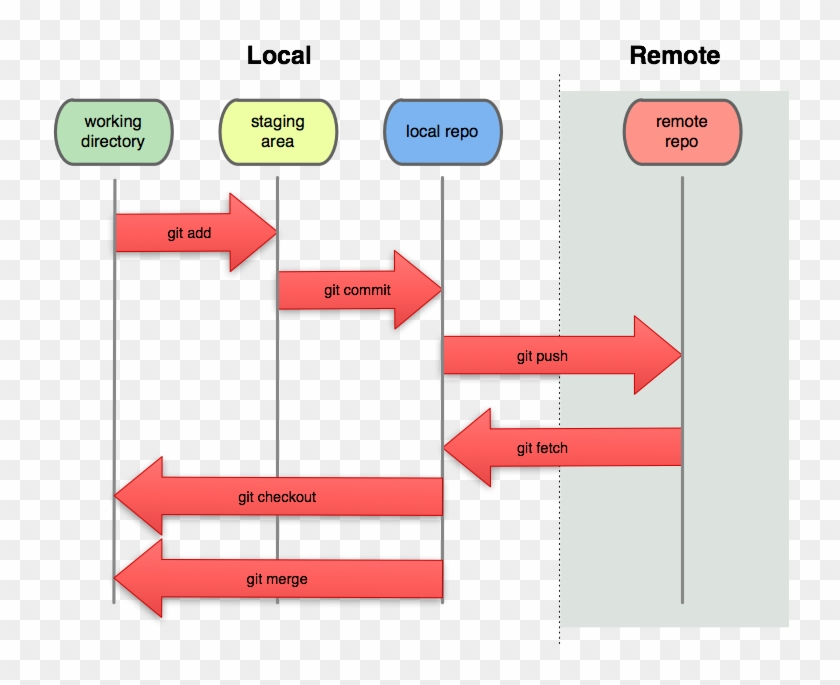
\includegraphics[width=0.8\textwidth]{images/tecnologie/comandi_git.png}
    \caption{Comandi di base di Git}
    \label{fig:git_workflow}
\end{figure}
Essenzialmente un workflow di base con \textbf{Git} prevede:
\begin{list}{-}{}
    \item \textbf{Clonare} un \gls{repository}{}, se già esistente;
    \item \textbf{Modificare} i file all'interno della \gls{working directory}{};
    \item \textbf{Stage} dei file, ovvero prepararli per il prossimo \textit{commit}, aggiungendoli alla \textit{staging area} con il comando \textit{git add};
    \item \textbf{Commit} dei file, ovvero versionarli, con il comando \textit{git commit}, i file così come son salvati nella \textit{staging area} vengono versionati all'interno del \gls{repository}{};
    \item \textbf{Push} delle modifiche sul \gls{repository}{} remoto.
\end{list}
\subsubsection{GitHub}
Per quanto riguarda il servizio di hosting che ha ospita il \gls{repository}{} remoto è stato utilizzato \textbf{GitHub}, andando a condividere 
i contenuti tra il mio account e quello del tutor aziendale (Figura \ref{fig:github}).\\
\begin{figure}[h]
    \centering
    
\includegraphics[width=0.4\textwidth]{images/tecnologie/logo_github.png}
    \caption{Logo di GitHub}
    \label{fig:github}
\end{figure}
\\
\textbf{GitHub} è una piattaforma di hosting per progetti software, che utilizza \textbf{Git} come sistema di controllo di versione e contiene tutti 
i file e i \gls{metadati}{} relativi alle modifiche validate lungo le fasi del progetto.\\
\pagebreak
\subsection{Documentazione}
Per quanto riguarda la redazione della documentazione, Sync Lab non ha uno standard prefissato e mi ha permesso di scegliere quale software utilizzare per la 
produzione dei documenti. La scelta è ricaduta su \textbf{LaTeX}, un linguaggio di markup per la preparazione di testi.\\
\subsubsection{LaTeX}
\textbf{LaTex}  è un sistema di composizione tipografica ampiamente utilizzato per la creazione di documenti di alta qualità. A differenza dei tradizionali editor di testo, LaTeX si basa su comandi di formattazione e struttura, consentendo agli utenti di concentrarsi sul contenuto del documento anziché sul suo aspetto visivo.\\
È stato sviluppato da Leslie Lamport negli anni '80 come estensione di TeX, un linguaggio e motore di composizione sviluppati da Donald Knuth (Figura \ref{fig:latex}).

\noindent \textbf{LaTeX} semplifica notevolmente la creazione di documenti complessi, grazie alla sua capacità di gestire automaticamente numerazione delle sezioni, citazioni bibliografiche, tabelle dei contenuti e molte altre funzionalità tipografiche avanzate.
L'ecosistema che \textbf{LaTeX} offre una vasta gamma di pacchetti e stili predefiniti che consentono di creare documenti sofisticati e professionali.
Per quanto riguarda la scelta dell'editor da utilizzare l'azienda non ha dato vincoli rilevanti, quindi la scelta è ricaduta su \textbf{TexLive}, un distribuzione \textbf{LaTeX} per sistemi operativi Linux e su \textbf{Texworks} come editor di testo.
\begin{figure}[h]
    \centering
    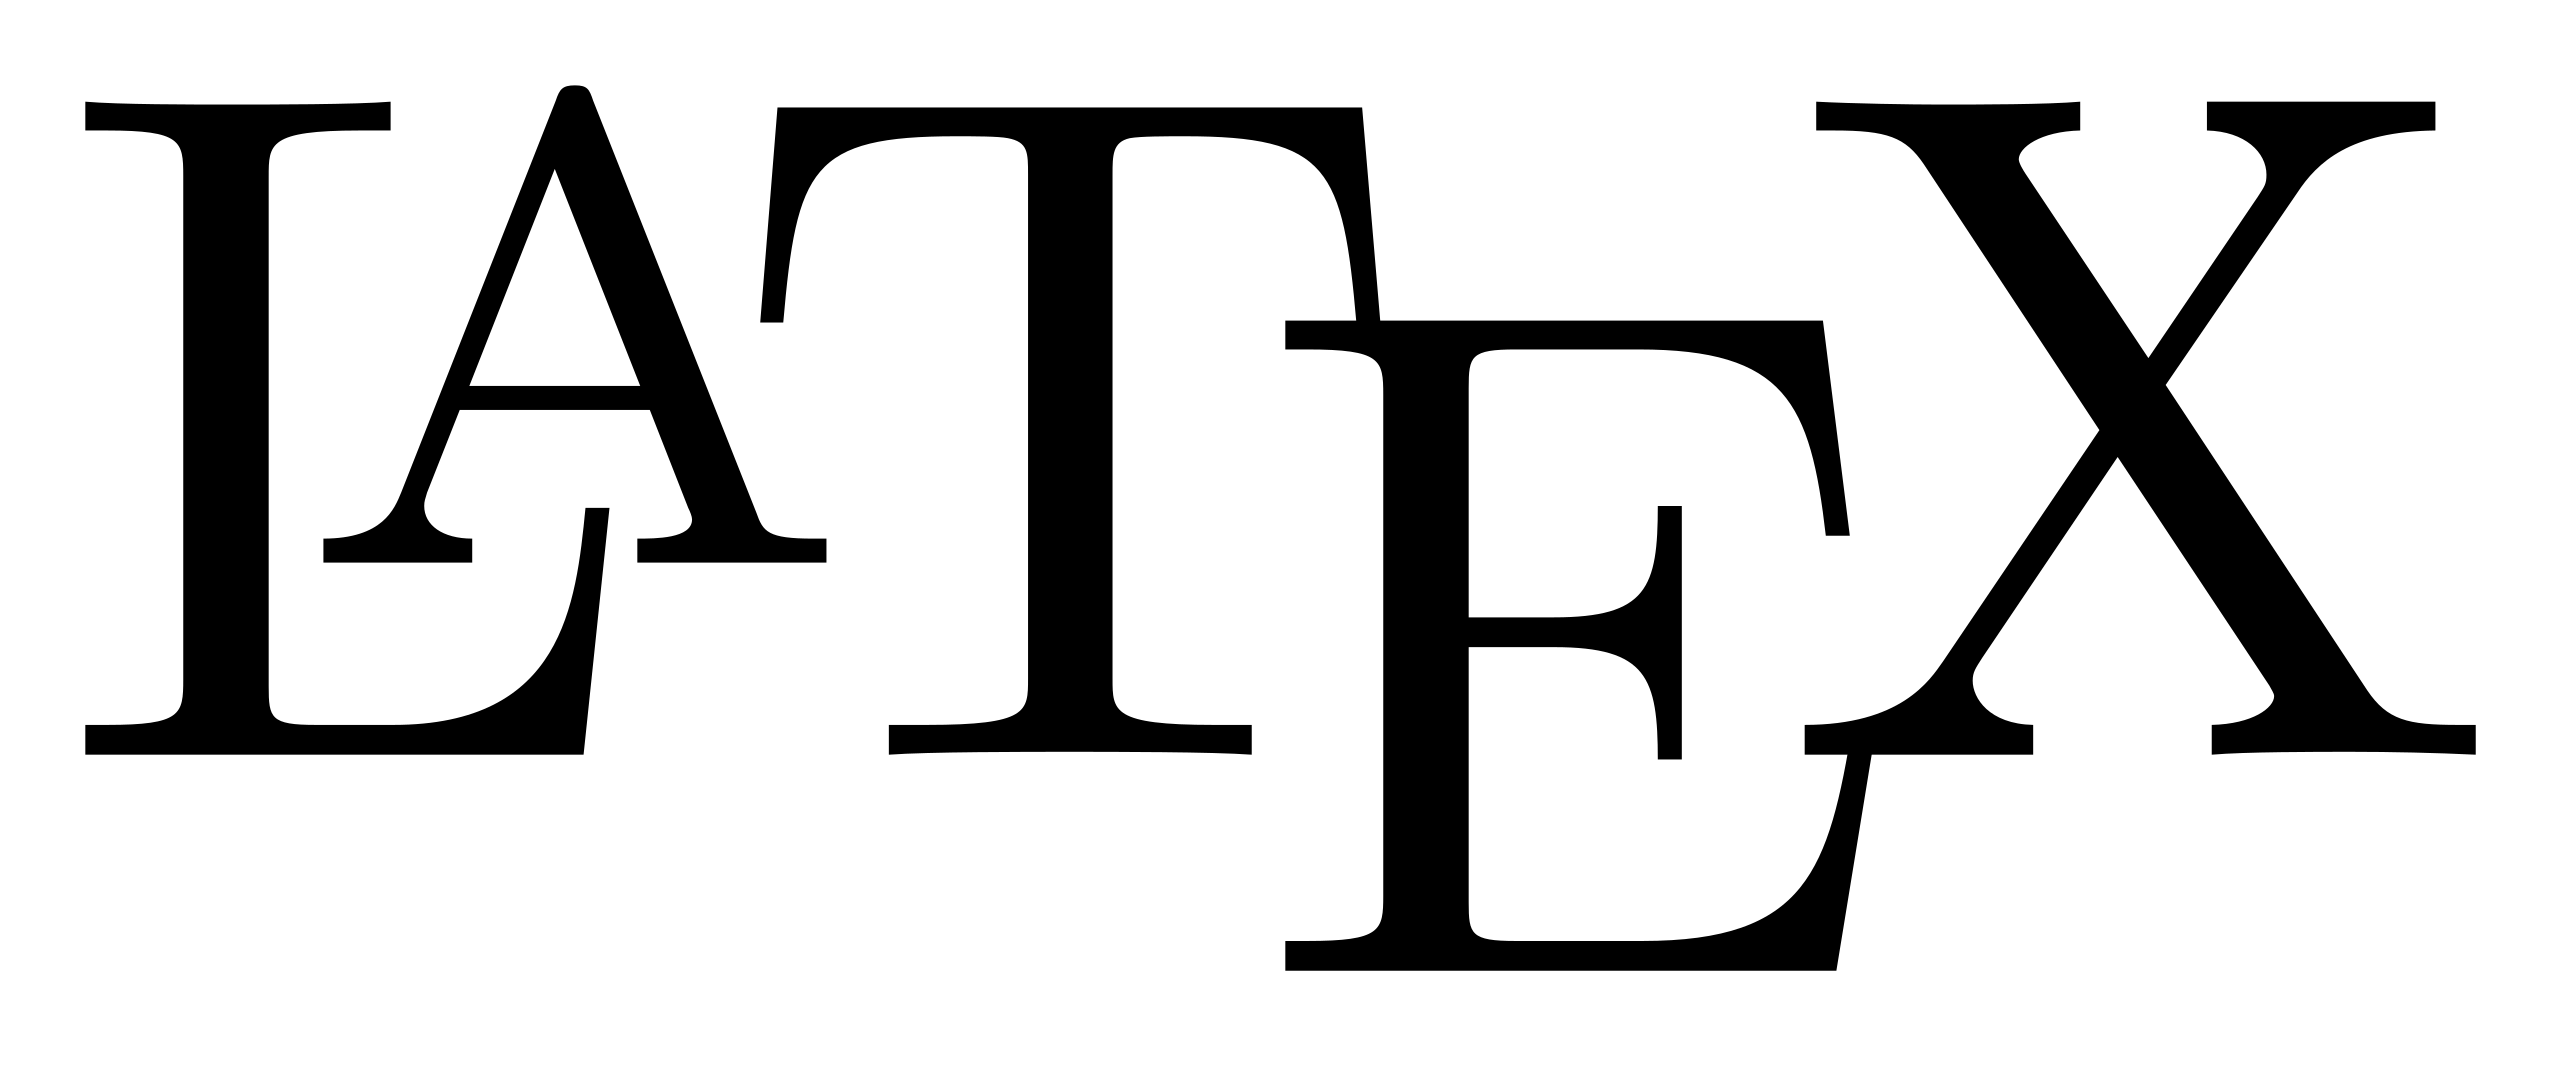
\includegraphics[width=0.3\textwidth]{images/tecnologie/logo_latex.png}
    \caption{Logo di LaTeX}
    \label{fig:latex}
\end{figure}
\subsection{Vincoli implementativi}
Per quanto riguarda l'implementazione del prototipo richiesto dall'azienda, non sono stati dati particolari vincoli implementativi,
se non che il prodotto finale debba essere eseguibile con Docker Compose e che metta in evidenza l'architettura richiesta. 
\newpage
\pagestyle{empty}
\null % o \mbox{} o \phantom{X}
\newpage
    \pagebreak
    \chapter{Analisi dei requisiti}\label{cap:analisi-requisiti}
    \pagebreak
    \chapter{Progettazione}\label{cap:progettazione}
    \pagebreak
    \chapter{Codifica e verifica}\label{ch:codifica_e_verifica}
    \pagebreak
    \chapter{Valutazioni e Conclusioni}
\label{cap:conclusioni}

\section{Consuntivo finale}

\section{Raggiungimento degli obiettivi}

\section{Conoscenze acquisite}

\section{Valutazione personale}


    \appendix

    \backmatter
    \printglossary[type=\acronymtype, title=Acronimi e abbreviazioni, toctitle=Acronimi e abbreviazioni]
    \printglossary[type=main, title=Glossario, toctitle=Glossario]

    \cleardoublepage
\chapter{Bibliografia}

\nocite{*}

% Print book bibliography
\printbibliography[heading=subbibliography,title={Riferimenti bibliografici},type=book]

% Print site bibliography
\printbibliography[heading=subbibliography,title={Siti web consultati},type=online]

\end{document}
